
\documentclass[11pt]{beamer}

% Packages ====================================================================
\usepackage{arev}
\usepackage[T1]{fontenc}
\usepackage[utf8]{inputenc}
\usepackage{float, afterpage, rotating, graphicx}
\usepackage{epstopdf}
\usepackage{longtable, booktabs, tabularx}
\usepackage{fancyvrb, moreverb, relsize}
\usepackage{eurosym, calc, chngcntr}
\usepackage{amsmath, amssymb, amsfonts, amsthm}
\usepackage{xcolor}
\usepackage{verbatim}
\usepackage{setspace}
\usepackage{appendixnumberbeamer}
\usepackage{subcaption}
\usepackage{ragged2e}
\usepackage[backend=biber, natbib=true, bibencoding=inputenc, bibstyle=authoryear-ibid, citestyle=authoryear-comp, maxcitenames=3, maxbibnames=10]{biblatex}
\setlength{\bibitemsep}{1.5ex}
\addbibresource{../refs.bib}
\hypersetup{colorlinks=true, linkcolor=., anchorcolor=., citecolor=., filecolor=., menucolor=., runcolor=., urlcolor=.}

% Commands =====================================================================
\DeclareMathOperator*{\argmin}{arg\,min}
\DeclareMathOperator*{\argmax}{arg\,max}
\renewcommand{\vec}[1]{\mathbf{#1}}
\def\newblock{\hskip .11em plus .33em minus .07em}
\newcommand{\bs}{\boldsymbol}
\newcommand{\N}{\mathbb{N}}
\newcommand{\cov}{\mathrm{cov}\thin}
\newcommand{\thin}{\thinspace}
\newcommand{\thick}{\thickspace}
\newcommand{\Lim}[1]{\raisebox{0.5ex}{\scalebox{0.8}{$\displaystyle \lim_{#1}\;$}}}
\newcommand{\vect}[1]{\mathbf{#1}}
\newcommand{\myfrac}[3][0pt]{\genfrac{}{}{}{}{\raisebox{#1}{$#2$}}{\raisebox{-#1}{$#3$}}}
\newcommand{\U}{\mathrm{U}} %Uniform Distribution
\newcommand{\D}{\mathrm{D}} %Dirichlet Distribution
\newcommand{\W}{\mathrm{W}} %Wishart Distribution
\newcommand{\E}{\mathrm{E}}     %Expectation
\newcommand{\Prob}{\mbox{Pr}}       %Expectation
\newcommand{\Iden}{\mathbb{I}}  %Identity Matrix
\newcommand{\Ind}{\mathrm{I}}   %Indicator Function
\newcommand{\Tau}{\mathcal{T}\thin}
\newcommand{\var}{\mathrm{var}\thin}
\newcommand{\plim}{\mathrm{plim}\thin}
\newcommand\indep{\protect\mathpalette{\protect\independenT}{\perp}}
\def\independenT#1#2{\mathrel{\rlap{$#1#2$}\mkern5mu{#1#2}}}
\newcommand{\notindep}{\ensuremath{\perp\!\!\!\!\!\!\diagup\!\!\!\!\!\!\perp}}%
\newcommand{\mc}{\multicolumn}
\newcommand{\ph}{\phantom}

\newcommand\Wider[2][3em]{%
\makebox[\linewidth][c]{%
  \begin{minipage}{\dimexpr\textwidth+#1\relax}
  \raggedright#2
  \end{minipage}%
  }%
}

% Colors =======================================================================
% short color names
% blues
\definecolor{lb}{HTML}{3498DB}
\definecolor{b}{HTML}{1565C0}
\definecolor{db}{HTML}{002080}
% greens
\definecolor{lg}{HTML}{B2EC5D}
\definecolor{g}{HTML}{55A868}
\definecolor{dg}{HTML}{2E7D32}
% yellows
\definecolor{ly}{HTML}{F9A825}
\definecolor{y}{HTML}{FF8F00}
\definecolor{dy}{HTML}{EF6C00}
% reds
\definecolor{lr}{HTML}{D84315}
\definecolor{r}{HTML}{C44E52}
\definecolor{dr}{HTML}{C62828}
% violet
\definecolor{lv}{HTML}{C71585}
\definecolor{v}{HTML}{9B59B6}
\definecolor{dv}{HTML}{6A1B9A}
% grey
\definecolor{ln}{HTML}{BDBDBD}
\definecolor{n}{HTML}{757575}
\definecolor{dn}{HTML}{616161}
% palettes
\definecolor{p1}{HTML}{4A6FAC}
\definecolor{p2}{HTML}{53A465}
\definecolor{p3}{HTML}{C04C50}
\definecolor{p4}{HTML}{7E6FAE}
\definecolor{p5}{HTML}{C8B571}
\definecolor{p6}{HTML}{62B1C8}
% brown
\definecolor{brown}{HTML}{4E342E}

% long color names
\definecolor{mm-lightblue}{HTML}{3498DB}
\definecolor{md-lightblue}{HTML}{0277BD}
\definecolor{mm-blue}{HTML}{002080}
\definecolor{md-blue}{HTML}{1565C0}
\definecolor{md-indigo}{HTML}{283593}

\definecolor{md-lime}{HTML}{9E9D24}
\definecolor{mm-lightgreen}{HTML}{B2EC5D}
\definecolor{md-lightgreen}{HTML}{558B2F}
\definecolor{mm-green}{HTML}{55A868}
\definecolor{md-green}{HTML}{2E7D32}
\definecolor{md-teal}{HTML}{00695C}

\definecolor{md-yellow}{HTML}{F9A825}
\definecolor{mm-gold}{HTML}{FFBF00}
\definecolor{md-amber}{HTML}{FF8F00}
\definecolor{md-orange}{HTML}{EF6C00}
\definecolor{md-deeporange}{HTML}{D84315}

\definecolor{mm-red}{HTML}{C44E52}
\definecolor{md-red}{HTML}{C62828}
\definecolor{violetred}{HTML}{C71585}

\definecolor{md-brown}{HTML}{4E342E}

\definecolor{md-pink}{HTML}{AD1457}
\definecolor{mm-violet}{HTML}{9B59B6}
\definecolor{md-purple}{HTML}{6A1B9A}
\definecolor{md-deeppurple}{HTML}{4527A0}

\definecolor{md-lightgrey}{HTML}{BDBDBD}
\definecolor{mm-gray}{HTML}{95A5A6}
\definecolor{md-grey}{HTML}{757575}
\definecolor{md-bluegrey}{HTML}{37474F}
\definecolor{md-darkgrey}{HTML}{616161}

\definecolor{sns-blue}{HTML}{4A6FAC}
\definecolor{sns-green}{HTML}{53A465}
\definecolor{sns-red}{HTML}{C04C50}
\definecolor{sns-violett}{HTML}{7E6FAE}
\definecolor{sns-beige}{HTML}{C8B571}
\definecolor{sns-lightblue}{HTML}{62B1C8}

\definecolor{mediumelectricblue}{rgb}{0.01, 0.31, 0.59}

% Design =======================================================================
% Here you define the main color of the presentation titles and structure elements
\colorlet{theme_color}{mediumelectricblue}
\setbeamertemplate{footline}[frame number]
\setbeamertemplate{navigation symbols}{}
\setbeamertemplate{frametitle}{\centering\vspace{1ex}\insertframetitle\par}
\setbeamerfont{alerted text}{series=\bfseries}
\setbeamerfont{title}{series=\bfseries}
\setbeamertemplate{section in toc}[circle]
\setbeamertemplate{subsection in toc}[square]
\setbeamercolor{structure}{fg=theme_color}
\setbeamercolor{alerted text}{use=structure,fg=structure.fg}


% Settings =====================================================================
\setstretch{1.5}
% Set Padding Around Equations
\AtBeginDocument{%
 \abovedisplayskip=-10pt plus 4pt minus 4pt
 \abovedisplayshortskip=0pt plus 3pt
 \belowdisplayskip=-10pt plus 4pt minus 4pt
 \belowdisplayshortskip=0pt plus 3pt
}

% Symbols =================================================================
\def\itemsymbol{$\blacktriangleright$}
\let\svpar\par
\let\svitemize\itemize
\let\svenditemize\enditemize
\let\svitem\item
\let\svcenter\center
\let\svendcenter\endcenter
\let\svcolumn\column
\let\svendcolumn\endcolumn
\def\newitem{\renewcommand\item[1][\itemsymbol]{\vfill\svitem[##1]}}%
\def\newpar{\def\par{\svpar\vfill}}%
\newcommand\stretchon{%
  \newpar%
  \renewcommand\item[1][\itemsymbol]{\svitem[##1]\newitem}%
  \renewenvironment{itemize}%
    {\svitemize}{\svenditemize\newpar\par}%
  \renewenvironment{center}%
    {\svcenter\newpar}{\svendcenter\newpar}%
  \renewenvironment{column}[2]%
    {\svcolumn{##1}\setlength{\parskip}{\columnskip}##2}%
    {\svendcolumn\vspace{\columnskip}}%
}
\usepackage{pifont}
% check mark in green
\newcommand{\cmark}{\textcolor{sns-green}{\ding{51}}}%
% red cross
\newcommand{\xmark}{\textcolor{sns-red}{\ding{55}}}%

% Structure slides==============================================================
\AtBeginSection[]{%
  \begin{frame}[plain, noframenumbering]
    \centering \huge\alert{\insertsection}\par
  \end{frame}}
\AtBeginSubsection[]{
  \begin{frame}[plain, noframenumbering]
    \centering \Large\alert{\insertsubsection}\par
  \end{frame}}

% Title and Author==============================================================
\author[Janoś Gabler]
{
{\bf Janoś Gabler}}

\begin{document}

\title{Why Structural Econometrics}
\date{\today}

\begin{frame}[plain, noframenumbering]
    \maketitle
    \note{~}
\end{frame}

\section{Introduction}

% Table of contents ============================================================
\begin{frame}[plain, noframenumbering]\frametitle{Outline}
  \hspace{1cm}\begin{minipage}{\textwidth}
    \tableofcontents[hideallsubsections]
  \end{minipage}
\end{frame}


\begin{frame}[c]\frametitle{Goals For This Lecture}
    \begin{itemize}
        \item Explain what structural econometrics is
        \item Show when it can be useful
        \item Relate it to use of models in other disciplines
        \item Look at one paper in detail
        \item Give you an intuition for structural modeling
    \end{itemize}
\end{frame}



\begin{frame}[c]\frametitle{Why Structural Econometrics?}
    \begin{itemize}
        \item Hierarchy of policy evaluations
        \begin{enumerate}
            \item[P1] Evaluate effect of a policy that has been implemented
            \item[P2] Predict effect of a policy that has been implemented in one environment would have in a different environment
            \item[P3] Predict the effect of a policy that has not yet been implemented (Ex-ante Evaluation)
        \end{enumerate}
        \item The main goal of structural econometrics is ex-ante Evaluation!
    \end{itemize}
\end{frame}


\begin{frame}[c]\frametitle{Models in Economics}
    \begin{itemize}
        \item Behavioral economists:
        \begin{itemize}
            \item Conceptual tool to organize thoughts
            \item Discipline thinking by mathematical rigor
            \item Rationalize results of experiments
        \end{itemize}
        \item Theorists:
        \begin{itemize}
            \item Uncover deep truths about human behavior
            \item Mechanism design
            \item Welfare theorems
        \end{itemize}
        \item Macroeconomists:
        \begin{itemize}
            \item ?
        \end{itemize}
        \item It's hard to tell what's a good model \ldots
    \end{itemize}
\end{frame}


\begin{frame}[c]\frametitle{Structural Models}
    \begin{itemize}
        \item Model = tool to predict causal effect of policies
        \item Can be used to design optimal policy
        \item Model is good if it predicts the effect reasonably well
        \item [$\rightarrow$] Unrealistic assumptions might be OK
        \item [$\rightarrow$] Channels of model are not always meaningful
    \end{itemize}
\end{frame}




\section{Models in Other Disciplines}
\subsection{Example 1: Car Manufacturers}

\begin{frame}[c]\frametitle{Example}
    \begin{itemize}
        \item Want to take an existing car and make it lighter
        \item There are many options:
        \begin{itemize}
            \item Replace steel by lighter materials
            \item Replace simple shapes by optimized profiles
            \item Make materials thinner
        \end{itemize}
        \item Each decision affects behavior in crash
        \item In the end, car needs to conform to standards
    \end{itemize}
\end{frame}


\begin{frame}[c]\frametitle{How Could Safety Be Assessed?}
    \begin{itemize}
        \item Experimental approach:
        \begin{itemize}
            \item Build (a few) prototypes for each design change
            \item Crash them at different speeds
            \item Assess safety for passengers
        \end{itemize}
        \item Problems:
        \begin{itemize}
            \item Prototypes cost a lot
            \item The process is very time consuming
            \item We haven't even tested combinations of changes!
            \item How would we ever find the the optimal new model?
        \end{itemize}
    \end{itemize}
\end{frame}


\begin{frame}[c]\frametitle{What is Actually Done?}
    \begin{itemize}
        \item Develop a computer model of cars
        \begin{itemize}
            \item Model = mapping from car to crash behavior
            \item Describe shape and material of each component
            \item Use properties of the materials to predict how the car reacts to a crash
            \item Make simplifying assumptions for speed reasons
        \end{itemize}
        \item Advantages:
        \begin{itemize}
            \item Reduce the number of costly experiments
            \item Try out multiple changes at a time
            \item Find the optimal combination of changes!
        \end{itemize}
    \end{itemize}
\end{frame}


\begin{frame}[c]\frametitle{How Do They Know it Works?}
    \begin{itemize}
        \item Actually build some cars and crash them
        \item Simulate crashes for the same cars
        \item Compare the results
        \item i.e. go back to the experimental approach
        \item This is called model validation
    \end{itemize}
\end{frame}


\subsection{Example 2: Climate Science}

\begin{frame}[c]\frametitle{Example}
    \begin{itemize}
        \item We want to predict effect of CO2 doubling on average air temperature in Germany
        \item Many things to consider
        \begin{itemize}
            \item Direct effect on atmospheric temperature
            \item Some extra heat is absorbed by oceans
            \item Feedback via change of ocean currents
        \end{itemize}
        \item Experimental approach is not possible
    \end{itemize}
\end{frame}


\begin{frame}[c]\frametitle{Conceptual Climate Model}
    \begin{figure}
        \includegraphics[width=\textwidth]{figures/climate_mechanisms.png}
    \end{figure}
\end{frame}


\begin{frame}[c]\frametitle{Abstractions and Simplifications}
    \begin{figure}
        \includegraphics[height=0.8\textheight]{figures/climate_abstractions.png}
    \end{figure}
\end{frame}


\begin{frame}[c]\frametitle{Equations}
    \begin{figure}
        \includegraphics[width=\textwidth]{figures/climate_equations.png}
    \end{figure}
\end{frame}



\begin{frame}[c]\frametitle{How to Calibrate This Model}
    \begin{itemize}
        \item Divide the model into components
        \begin{itemize}
            \item Atmospheric model
            \item 2 layer ocean model
        \end{itemize}
        \item Calibrate components by lab experiments
        \begin{itemize}
            \item Ocean = bathtub
        \end{itemize}
        \item Measure initial conditions as precisely as possible
        \begin{itemize}
            \item More than 40 000 weather stations worldwide
            \item Sensors to measure ocean temperature
        \end{itemize}
    \end{itemize}
\end{frame}


\begin{frame}[c]\frametitle{How Do They Know it Works?}
    \begin{itemize}
        \item Validate subcomponents
        \item Quantify uncertainty around initial conditions
        \item Quantify uncertainty around lab calibrated parameters
    \end{itemize}
\end{frame}


\subsection{Summary}

\begin{frame}[c]\frametitle{Summary I}
    \begin{itemize}
        \item Engineers
        \begin{itemize}
            \item Can experiment
            \item Use models to need fewer experiments
            \item Calibrate and validate models with experimental data
        \end{itemize}
        \item Climate scientists
        \begin{itemize}
            \item Can only do very simplified experiments
            \item Use models to replace real experiments
            \item Calibrate and validate subcomponents
        \end{itemize}
    \end{itemize}
\end{frame}



\begin{frame}[c]\frametitle{Summary II}
\begin{itemize}
    \item In both cases, models are:
    \begin{itemize}
         \item Extremely simplified (``all models are wrong'')
         \item Have a clear purpose (prediction)
         \item Might be wrong but good enough for that purpose
     \end{itemize}
     \item Economists are between the two
     \begin{itemize}
         \item Experimentation is more difficult than for engineers
         \item Macro-experiments are sometimes possible
     \end{itemize}
\end{itemize}
\end{frame}


\section{An Example of a Structural Model}

\subsection{Background}

\begin{frame}[c]\frametitle{The PROGRESA Program}
    \begin{itemize}
        \item \cite{Todd2006} evaluates the Conditional Cash Transfer (CCT) PROGRESA
        \item first Latin American CCT program
        \item Eligible mothers get cash if children go to school and health checkups
        \item Transfers start at $3^\text{rd}$ grade and end after $9^\text{th}$ grade
        \item Benefit increases with grade and is higher for girls
    \end{itemize}
\end{frame}



\begin{frame}[c]\frametitle{Transfer Schedule}
\vspace{-0.5cm}
\center{\resizebox{0.6\textwidth}{!}{
\begin{tabular}{lccc}
\toprule
                &               & \multicolumn{2}{c}{Monthly Payment in Pesos}  \\
                \cmidrule(r){3-4}
School Level    & Grade         & Females       & Males                         \\
\midrule
Primary         & 3             & 70            & 70                            \\
                & 4             & 80            & 80                            \\
                & 5             & 105           & 105                           \\
                & 6             & 135           & 135                           \\
Secondary       & 1             & 210           & 200                           \\
                & 2             & 235           & 210                           \\
                & 3             & 255           & 225                           \\
\bottomrule
\end{tabular}}}
\vspace{1cm}

\begin{itemize}
    \item For US-Dollars, divide by 10
\end{itemize}
\end{frame}


\begin{frame}[c]\frametitle{Hypothesized Effects of CCTs}
    \begin{columns}[t]
        \begin{column}{0.4\textwidth}
            \textcolor{sns-green}{
            \textbf{Positive}}
            \begin{itemize}
                \item \textcolor{sns-green}{Increase human capital via school attendance}
                \item \textcolor{sns-green}{Improve child health}
                \item \textcolor{sns-green}{Alleviate extreme poverty}
            \end{itemize}
        \end{column}
        \begin{column}{0.4\textwidth}
            \textcolor{sns-red}{\textbf{Negative}}
            \begin{itemize}
                \item \textcolor{sns-red}{Negative incentives on fertility decisions of young women}
            \end{itemize}
        \end{column}
    \end{columns}
\end{frame}


\begin{frame}[c]\frametitle{The Field Experiment}
    \begin{itemize}
        \item Random Assignment of:
        \begin{itemize}
            \item 320 treatment villages
            \item 186 control villages
        \end{itemize}
        \item In treatment villages, about 50 \% of households are eligible
        \item Pre-intervention data collected before March 1998
        \item Post-intervention data collected until end of 1999
    \end{itemize}
\end{frame}


\subsection{Policy Questions}


\begin{frame}[c]\frametitle{What Can We Learn from the Experiment?}
\pause
What is the ATT of the implemented transfer scheme on school attainment \pause one year after the intervention \pause if the policy is introduced as a surprise  \pause but announced to be permanent?
\end{frame}


\begin{frame}[c]\frametitle{And Which Can't?}
\begin{itemize}
    \item What is the most \alert{efficient transfer scheme}?
    \item What is the effect of that policy if it is already \alert{in place when people take fertility decisions}?
    \item What is the effect on \alert{total school attainment}?
\end{itemize}
\end{frame}


\begin{frame}[c]\frametitle{Summary of the Paper}
\begin{itemize}
    \item Answers the questions that can't be answered by the experiment
    \item Requires a structural model
    \item ``no consensus on what is a reasonable model''
    \begin{itemize}
        \item Estimate model on control group data
        \item Use it to predict the effect of the experiment
        \item Validate model on treatment group
    \end{itemize}
    \item One of the first papers to address and implement model validation in a systematic way
\end{itemize}
\end{frame}


\subsection{A Model of Schooling Choices and Fertility}

\begin{frame}[c]\frametitle{Type of Model}
    \begin{itemize}
        \item Finite Horizon \alert{Discrete Choice Dynamic Programming} (DCDP) Model
        \item \alert{Intuitively}: ``\textit{\small{a behavioral economic model that can be described as sequential discrete choice optimization problems constrained by resource limitations and imperfect information about future events.}}''
        \item Widely applied for ex-ante policy evaluation
        \item Models the decision making process of individuals
        \item After policy, decisions change but decision making process does not!
    \end{itemize}
\end{frame}



\begin{frame}[c]\frametitle{Choice Set}
    \begin{itemize}
        \item The model has T periods
        \item In each period, households decide:
        \begin{itemize}
            \item Whether to become pregnant or not
            \item For each child, decide whether:
            \begin{itemize}
                \item Child stays at home
                \item Child goes to school
                \item Child works and earns income
            \end{itemize}
        \end{itemize}
        \item In each fertile period there are $2 \cdot 3^{n}$ options, where $n$ is the number of children
    \end{itemize}
\end{frame}


\begin{frame}[c]\frametitle{Rewards and Constraints}
    \begin{itemize}
        \item Immediate utility depends on:
        \begin{itemize}
            \item Consumption
            \item Pregnancy and birth history
            \item Schooling history for each child
            \item Children at home
            \item Distance to school
            \item Shocks
        \end{itemize}
        \item Constraints
        \begin{itemize}
            \item Consumption = (exogenous) parent income + (endogenous) child labor income
        \end{itemize}
    \end{itemize}
\end{frame}


\begin{frame}[c]\frametitle{State Space}
    \begin{itemize}
        \item \alert{Definition}: set of all factors, known to the individual, that affect current rewards or the probability distribution of any of the future rewards.

        \item The state space contains:
        \begin{itemize}
            \item Birth histories of sons and daughters
            \item School histories of sons and daughters
            \item Age of parents and age at marriage
            \item Distance to secondary school and city
            \item Current preference shocks (unobserved)
            \item Types (permanent heterogeneity, unobserved)
        \end{itemize}
        \item The state space is huge
    \end{itemize}
\end{frame}


\subsection{Identification of the Policy Effect From Observational Data}


\begin{frame}[c]\frametitle{Identification of the Policy Effect}
\begin{columns}
\begin{column}{.95\textwidth}
\begin{itemize}

    \item \alert{Best Case}: exogenous variation in tuition costs

    \item \alert{Instead}: exploit variation in child wages

    \item \alert{Problem}: only observe wages if children work

    \item \alert{Solution}:
    \begin{itemize}
         \item Estimate the wage offer distribution
        \item Model is identified, if there is a variable that affects wage offers but not parents' preference for schooling
        \item Authors use distance to next city
     \end{itemize}
\end{itemize}
\end{column}
\begin{column}{0.05\textwidth}
\begin{figure}
    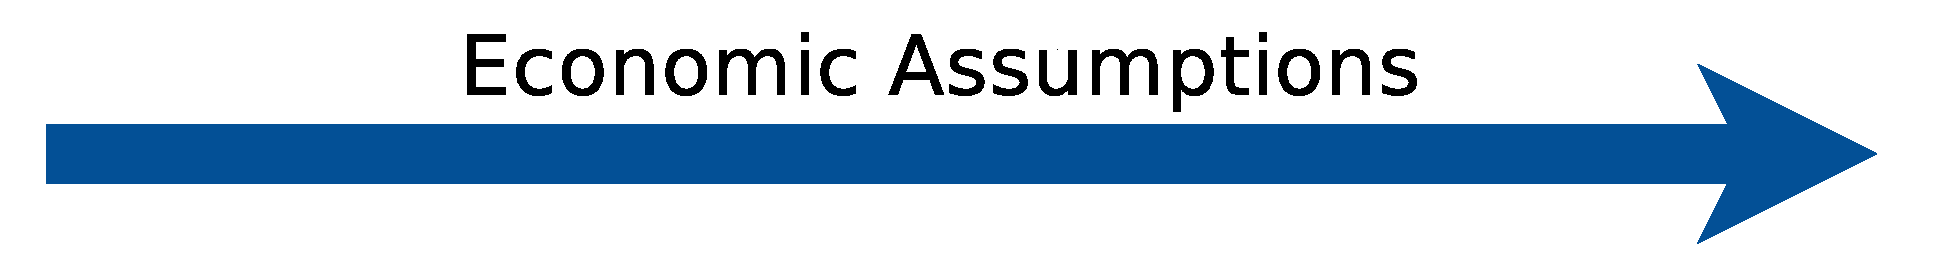
\includegraphics[angle=270,origin=c,height=0.37\textheight]{graphs/Diagram1.eps}
\end{figure}
\end{column}
\end{columns}
\end{frame}


\begin{frame}[c]\frametitle{Convenience Assumptions}
\begin{itemize}
    \item Distributional assumptions on unobservables
    \item Functional form assumptions on utility functions
    \item Not only needed for estimation, but even for identification
    \item Model can be estimated by maximum likelihood
\end{itemize}
\end{frame}



\subsection{Model Validation}

\begin{frame}[c]\frametitle{What Is Meant By Validation}
    \begin{itemize}
        \item In-sample goodness of fit measures can't check model's ability to predict counterfactuals
        \item Instead: use model to predict effects of policies not observed in the estimation sample
        \item Compare predictions with experimental treatment effects
        \item If this works, consider the model to be validated with respect to that policy question
    \end{itemize}
\end{frame}


\begin{frame}[c]\frametitle{Use the Model to Predict Treatment Effects}
    \begin{itemize}
        \item Closer look at the budget constraint in the treatment group:
    \end{itemize}
        \begin{equation}
            C(t) = y_p(t) + \sum_{n = 1}^{N} y_n(t) \mathbb{I}_{\{\text{n works}\}} + \textcolor{mediumelectricblue}{\tau_n(t) \mathbb{I}_{\{\text{n at school}\}}}
        \end{equation}
    \begin{itemize}
        \item This can be used for counterfactual simulation
        \item To do so, use 200 simulation draws per family
        \item In what follows, this is used to:
        \begin{itemize}
            \item Predict experimental treatment effects
            \item Predict choices
            \item Answer the policy questions
        \end{itemize}
    \end{itemize}
\end{frame}


\begin{frame}[c]%\frametitle{Actual and Predicted Treatment Effects}
    \begin{figure}
        \caption{\textcolor{mediumelectricblue}{Actual and predicted treatment effects}}
        \includegraphics[width=\textwidth]{graphs/table0.eps}
    \end{figure}
    \vspace{-0.8cm}
    \pause
    \begin{itemize}
        \item Effects of the policy on school attendance rates after 1 year
        \item Children aged 12 to 15
        \item Bars show $\pm 1$ Standard Error
    \end{itemize}
\end{frame}

\begin{frame}[c]%\frametitle{Actual and Predicted Choices}

    \begin{figure}
        \centering
        \caption{Actual And Predicted Choices}
        \begin{subfigure}[c]{0.5\textwidth}
            \centering
            \includegraphics[width=\textwidth]{graphs/girls_table1.eps}
            \caption{Girls}
        \end{subfigure}%
        \begin{subfigure}[c]{0.5\textwidth}
            \centering
            \includegraphics[width=\textwidth]{graphs/boys_table1.eps}
            \caption{Boys}
        \end{subfigure}

    \end{figure}
    \begin{itemize}
        \item Children aged 12 to 15
        \item Deviations between actual and predicted group percentages
        \item Overall pretty good!
    \end{itemize}
\end{frame}




\begin{frame}[c]%\frametitle{N-Years Ahead Predictions}
\begin{figure}
        \centering
        \caption{Actual and Predicted Schooling N-Years Ahead}
        \begin{subfigure}[c]{0.5\textwidth}
            \centering
            \includegraphics[width=\textwidth]{graphs/girls_table2_school.eps}
            \caption{Girls}
        \end{subfigure}%
        \begin{subfigure}[c]{0.5\textwidth}
            \centering
            \includegraphics[width=\textwidth]{graphs/boys_table2_school.eps}
            \caption{Boys}
        \end{subfigure}
\end{figure}
\begin{itemize}
    \item Predictions only based on household characteristics at marriage!
\end{itemize}
\end{frame}


\begin{frame}[c]%\frametitle{title}
    \begin{figure}
        \centering
        \caption{Actual and Predicted Pregnancy Rate N-Years Ahead}
            \includegraphics[width=0.5\textwidth]{graphs/girls_table2_pregnancy.eps}
\end{figure}

\begin{itemize}
    \item Predictions only based on household characteristics at marriage!
\end{itemize}
\end{frame}


%\begin{frame}[c]\frametitle{Should You Believe the Results Now?}
%\begin{itemize}
%    \item Decide for yourself!
%    \item The important thing is:
%    \begin{itemize}
%        \item To do so, you need expert knowledge about the school system
%        \item You don't have to understand the statistical assumptions in detail
%    \end{itemize}
%    \item This gives policy makers a much better chance to assess credibility
%\end{itemize}
%\end{frame}


\subsection{Answers to Policy Questions}

\begin{frame}[c]\frametitle{Treatment Effects in Short and Long Run}
    \center{
    \resizebox{0.7\textwidth}{!}{    \begin{tabular}{lcccc}
    \toprule
                    & \multicolumn{2}{c}{Girls} & \multicolumn{2}{c}{Boys} \\
                    \cmidrule(r){2-3}         \cmidrule(r){4-5}
                    & Short-run & Long-run      & Short-run & Long-run      \\
                    & effect    & effect        & effect    & effect        \\
    \midrule
    Control group   &           &               &           &               \\
    1997            &   10.9    &   11.9        &   10.7    &       12.0    \\
    1998            &   11.2    &   12.3        &   11.4    &       12.7    \\
    Treatment group &           &               &           &               \\
    1997            &   11.2    &   12.3        &   11.3    &       12.4    \\
    1998            &   11.7    &   12.7        &   12.1    &       12.4    \\
    \bottomrule
    \end{tabular}
}}
    %\end{centering}
    \vspace{0.7cm}
    \begin{itemize}
        \item Effects of the policy on school attendance rates
        \item Long: program is in place since marriage!
        \item Long effects slightly larger than short run effects
    \end{itemize}
\end{frame}


\begin{frame}[c]\frametitle{Effects on Completed Schooling}
    \begin{centering}
        \resizebox{\textwidth}{!}{    \begin{tabular}{lcccc}
    \toprule
                    & \multicolumn{2}{c}{Girls} & \multicolumn{2}{c}{Boys} \\
                    \cmidrule(r){2-3}         \cmidrule(r){4-5}
                    & No subsidy & Subsidy      & No subsidy & Subsidy      \\
    \midrule
    Mean schooling  & 6.29      & 6.83          & 6.42      & 6.96          \\
    \% completing grade 6 or more & 75.8 & 82.2 & 78.8      & 83.3          \\
    \% completing grade 9 or more & 19.8 & 25.9 & 22.8      & 28.0          \\
    \bottomrule
    \end{tabular}
}
    \end{centering}
\end{frame}


\begin{frame}[c]\frametitle{Alternative Transfer Schedules}
    \begin{itemize}
        \item The authors simulate several alternative subsidies
        \item A cost neutral shift of transfers towards the higher grades, makes the treatment effect about 25 \% larger
        \item This was to be expected, since school attendance is universal in earlier grades
        \item \alert{Careful}: The outcome variable is only completed schooling; Positive effects on cognitive and non-cognitive skills through other parental investments are not included!
    \end{itemize}
\end{frame}


\begin{frame}[c]\frametitle{Summary of the Workflow}
    \begin{itemize}
        \item Specify explicit economic model of decision making
        \item Estimate the model on data
        \item Use estimates to simulate effect of policies
        \item Model is good if it predicts policies well
        \item Ideally, shown by validation through a policy experiment
    \end{itemize}
\end{frame}


\section{Some Notes on Structural Econometrics}


\begin{frame}[c]\frametitle{Why Are Individuals Optimizing}
    \begin{itemize}
        \item Reason 1: We believe in utility maximization
        \item Reason 2: People might behave close to optimal without optimizing
        \item Example:
            \begin{itemize}
                \item A new tax policy is implemented
                \item Some people find that after the change it's better to retire earlier
                \item They talk to others about what worked for them
                \item Over time, people converge to the optimum
                \item Basic argument: Swarm intelligence
            \end{itemize}
    \end{itemize}
\end{frame}


\begin{frame}[c]\frametitle{Wouldn't Almost-Optimization be Enough?}
    \begin{itemize}
        \item \cite{Lumsdaine1990} estimates three models of retirement
        \begin{enumerate}
            \item Standard DCDP model with dynamic optimization
            \item Option value model that is similar to the DCDP model but replaces the Emax function by the maxE function and thus simplifies the computational burden considerably.
            \item A static probit model.
        \end{enumerate}
        \item Validate all three models experimentally
        \item 1 and 2 are equally good
        \item Absolutely no impact on later literature!
    \end{itemize}
\end{frame}


\begin{frame}[c]\frametitle{Structural Econometrics and Experiments}
    \begin{itemize}
        \item Experiments can help structural Economists
        \begin{itemize}
            \item Cleaner Identification
            \item Validation
            \item \cite{Wolpin2013} discusses trade-offs
        \end{itemize}
        \item Structural models can help experimentalists
        \begin{itemize}
            \item Design the right experiment to identify effect of interest
            \item Model helps to organize thoughts \citep{DellaVigna2017a}
        \end{itemize}
    \end{itemize}
\end{frame}


\begin{frame}[c]\frametitle{Structural Econometrics and Machine Learning (ML)}
    \begin{itemize}
        \item Models are tools to predict effect of policies
        \item Machine Learning is great at prediction
        \item It makes less assumptions on behavior
        \item Why not use it instead?
        \pause
        \item ML predicts well as long as Data Generating Process does not change
        \item Structural Model uses theory to identify policy effect from surrogate variation in the data
    \end{itemize}
\end{frame}


\begin{frame}[c]\frametitle{What can We Learn from ML}
    \begin{itemize}
        \item Use (possibly non-random) holdout samples
        \item Cross validation techniques
        \item Modern Hardware (GPUs, TPUs, \ldots)
        \item Algorithmic improvements
        \item Function approximation methods
    \end{itemize}
\end{frame}


\section{Summary}


\begin{frame}[c]\frametitle{Summary}
\begin{itemize}
    \item Economists use models for various purposes
    \item Conceptual Tool, discipline thinking, Understanding behavior
    \item Other disciplines use models as prediction tools
    \begin{itemize}
        \item Opens the possibility to validate a model
    \end{itemize}
    \item Structural Econometrics bridges that gap
    \item Simplifying assumptions are ok, as long as you validate
    \item Good example: \cite{Todd2006}

\end{itemize}
\end{frame}







\appendix
\begin{frame}[allowframebreaks]
    \frametitle{References}
    \renewcommand{\bibfont}{\normalfont\footnotesize}
    \printbibliography
\end{frame}

\end{document}


